\documentclass[10pt,a4paper]{article}
\usepackage[utf8]{inputenc}
\usepackage[francais]{babel}
\usepackage[T1]{fontenc}
\usepackage{amsmath}
\usepackage{amsfonts}
\usepackage{amssymb}
\usepackage{graphicx}
\usepackage{epstopdf}
\usepackage{fancyhdr}
\pagestyle{fancy}
\usepackage{cite}


\renewcommand{\headrulewidth}{1pt}
\fancyhead[R]{} 
\fancyhead[L]{\textit{\leftmark}}

\addtolength{\hoffset}{-1.5cm}
\addtolength{\textwidth}{3.5cm}

\title{Projet MDI 343 \\
Systèmes de recommandation}
\author{Nicolas Keriven et Jean-Baptiste Alayrac}

\begin{document}
\maketitle

\hrulefill
\vspace{2cm}

% Si on veut mettre un abstract

%\renewcommand{\abstractname}{Résumé}
%\begin{abstract}
%
%
%\end{abstract}

% Figure 
%\begin{center}
%\begin{figure}[ht!]
%\includegraphics[width=\columnwidth]{fig/name.extension}
%\caption{\label{lab} titre}
%\end{figure}
%\end{center}

\newpage
\tableofcontents

\section*{Introduction}
\addcontentsline{toc}{section}{Introduction}
 
\newpage


\section{Présentation du problème et notations}

Le cadre général de la problématique de recommandation est de relier des utilisateurs à des produits. Dans cette partie nous présentons tout d'abord les méthodes les plus utilisées actuellement pour les système de recommandations avant de nous concentrer sur la méthode que nous avons approfondie.

\subsection{Différentes méthodes}

Actuellement, il existe deux principales approches afin de  créer un système de recommandation. La première approche est appelée \textit{content filtering} alors que la seconde est nommée \textit{collaborative filtering}

\subsubsection*{\textit{Content filtering} (ou filtrage par contenu)}

Cette méthode vise à caractériser la nature de chaque utilisateur ainsi que de chaque produit afin d'en dégager un profil le plus précis possible. Pour un utilisateur, cela peut être son pays d'origine, son âge... Pour un produit, par exemple un film, cela peut être son genre, son box-office... Les algorithmes ont alors pour tâche d'associer des profils d'utilisateurs avec des profils de produits. Le projet Music Genome Project, utilisé notamment dans la radio Pandora.com utilise de telles méthodes afin de proposer du contenu aux utilisateurs. Chaque musique est alors caractérisée par des centaines d'attributs assimilable à des "gènes". 


\subsubsection*{\textit{Collaborative filtering} (ou filtrage collaboratif)}

L'autre méthode se base essentiellement sur des avis passés (implicites ou explicites) d'utilisateurs à propos de produits. La méthode de \textit{collaborative filtering} analyse les liens qui existent entre utilisateurs et produits via la connaissance de votes passés afin de proposer de nouvelles associations utilisateur/produit. L'avantage principal de cette méthode par rapport à celle de \textit{content filtering} est qu'ici il n'y a nul besoin de connaître le produit ou les utilisateurs à priori. Par contre cette méthode connait le problème du \textit{cold start}, i.e., elle est incapable de traiter l'arrivée d'un nouveau produit ou d'un nouveau utilisateur. Afin de la faire fonctionner il faut posséder un nombre déjà conséquents d'avis de chaque utilisateurs et pour chaque produits.

Dans ce contexte de \textit{collaborative filtering} il existe à nouveau deux principales méthodes. La première est connue sous le nom de \textit{neighborhood method}, la deuxième se concentre autour de \textit{latent factor models}.

\begin{figure}[ht!]
\begin{center}
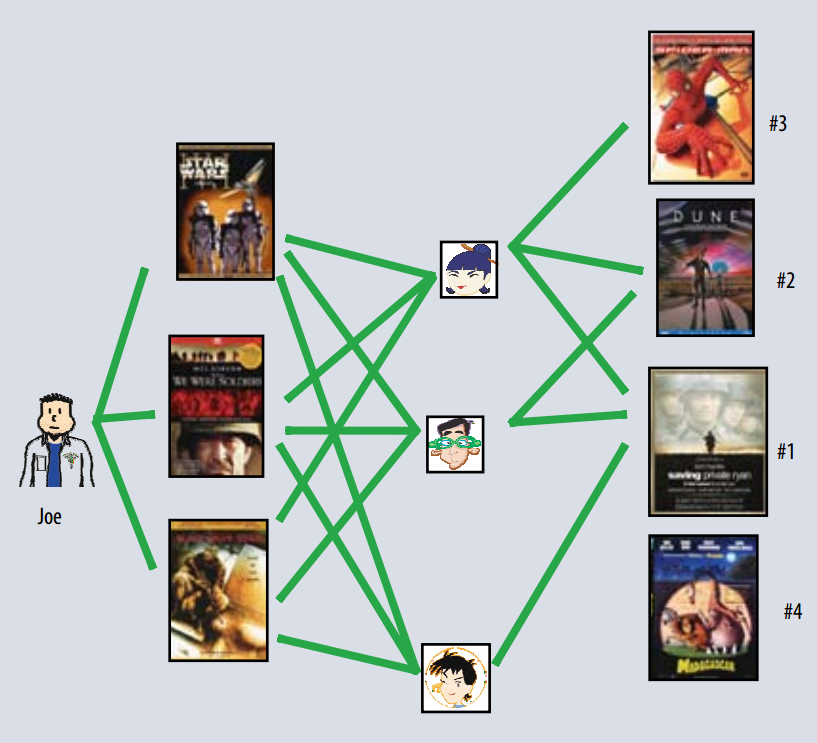
\includegraphics[height=5cm]{fig/neighboor_representation.png}
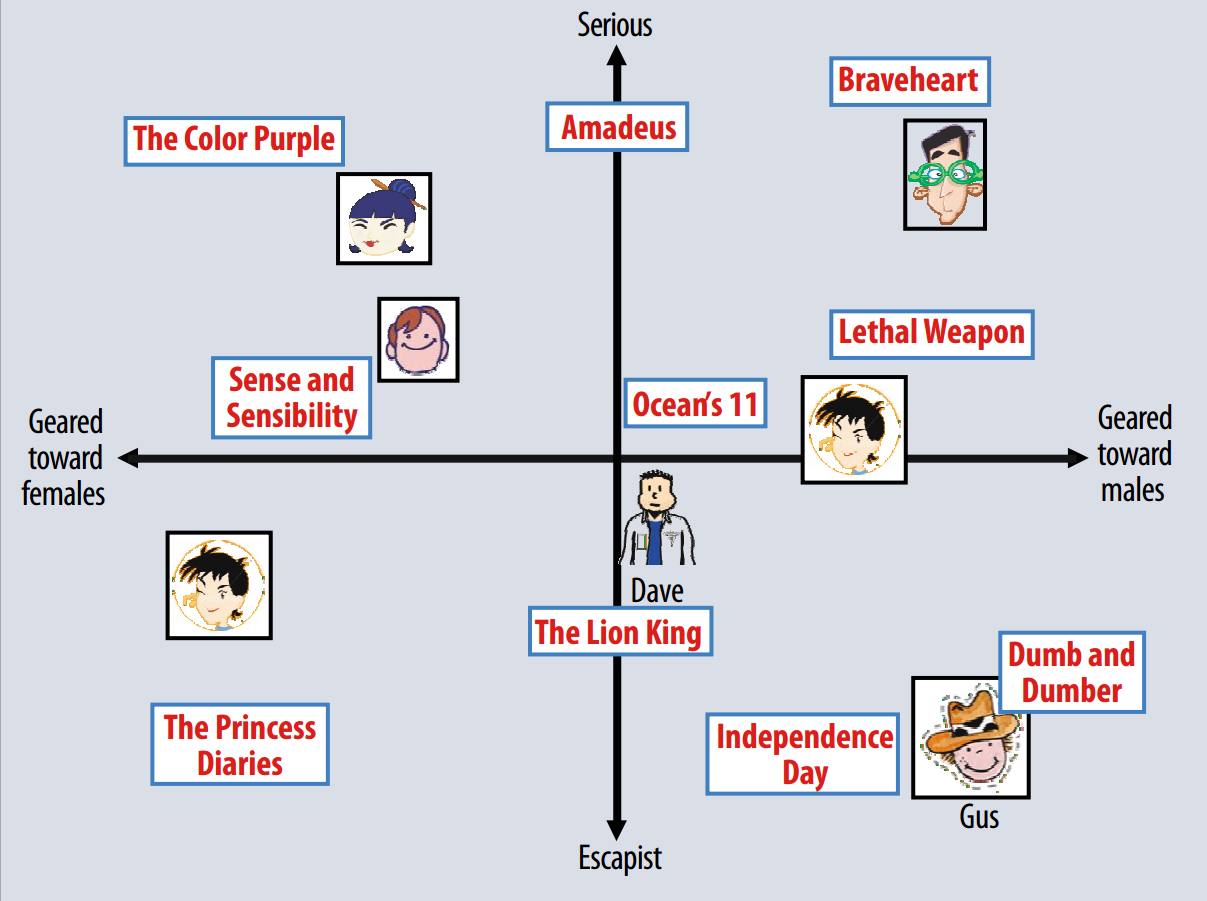
\includegraphics[height=5cm]{fig/factor_representation.png}
\caption{\label{nmet} A gauche : \textit{neighborhood methods}, A droite : \textit{Latent factor models}}
\end{center}
\end{figure}


\paragraph{\textit{Neighborhood methods}}

La principale idée est d'essayer de modéliser les relations qui existent entre les utilisateurs d'une part ou les produits d'autre part. Partons de l'approche produit. Supposons qu'on veuille prédire la note que va mettre un utilisateur à un nouveau produit A. On va alors regarder comment cet utilisateur a noté les produits identifiés comme étant des produits voisins de A, afin de prédire la note qu'il va mettre sur ce nouvel objet. Sur la gauche de la Figure \ref{nmet}, on a représenté l'approche utilisateur où l'on a d'abord trouvé un voisinage de l'utilisateur Joe afin de lui conseiller de nouveaux films (dans ce cas le premier film conseillé serait \textit{Il faut sauver le soldat Ryan}).

\paragraph{\textit{Latent factor model}}

Cette dernière approche est celle que nous avons choisi d'étudier plus en détails. L'idée derrière cette méthode est d'essayer est d'essayer de déterminer des \textit{facteurs latents} qui seront les dimensions d'un espace dans lequel on pourra plonger à la fois les utilisateurs et les produits. Cet espace sera directement déduit de la structure des votes qui est le lien entre utilisateurs et produits. L'idée ensuite est de pouvoir rassembler un utilisateur et un film qui seront proches dans cet espace. 

Ces facteurs latents peuvent être parfois interprétables. Par exemple une dimension pourront représenté le fait pour un film d'être une comédie. Les points maximaux seront alors considérés comme des comédies alors que les points minimaux pourront être des drames. La position d'un utilisateur sur cet axe témoignera alors de la propension de celui-ci à aimer ce genre. 

Cependant parfois ces facteurs ne sont pas interprétables directement, ce qui donne une certaine richesse au modèle. Cette méthode permet en effet de détecter des tendances qui n'aurait pas été prévisible à la main.

Sur la droite de la Figure 2 on a représenté cette approche pour 2 facteurs latents. De cela on peut prédire que l'utilisateur en haut à droite du graphique va certainement adorer le film \textit{Braveheart} alors qu'il va probablemnet détester le film \textit{The Princess Diaries}.

\subsection{Factorisation de matrice et notations}

Nous allons voir qu'une méthode afin de calculer ces facteur latents est de factoriser la partie connue de la matrice de notes $\textbf{M}$. On rappelle que $\textbf{M}_{u,i}$ est la note qu'a mis l'utilisateur $u$ au produit $i$ ($u$ pour \textit{user} et $i$ pour \textit{item}). Dans le cas où l'on a $n_u$ utilisateurs et $n_i$ produits cette matrice est donc de taille $n_u\times n_i$. Le gros obstacle est que cette matrice de notation est parcimonieuse, en effet bien souvent on ne possède qu'un certain nombre de produits pour lequel l'utilisateur a voté. Dans la suite on note $\Omega$ le set d'indices pour lequel la notation est connue. On a donc $|\Omega|\ll n_u\times n_i$. 

L'idée va alors être de trouver une matrice $\textbf{X}$ qui va être \textit{proche dans un certain sens} de l'information contenue dans la matrice $\textbf{M}$ et qui va pouvoir s'écrire de manière factorisé :

$$ \textbf{X} = LR^* $$

où $L \in \mathbb{R}^{n_u\times r}$ et $R \in \mathbb{R}^{n_i\times r}$ où $r$ est le nombre de facteurs latents que l'on recherche. Ainsi la ligne $u$ (resp. $i$) de la matrice $L$ (resp. $R$) va représenter la position dans l'espace des facteurs latents de l'utilisateur $u$ (resp. produit $i$). Le produit scalaire de ces deux vecteurs va donc représenter la propension de l'utilisateur $u$ a aimé le produit $i$. 

Maintenant essayons de décrire de manière plus mathématique la notion de \textit{proche dans un certain sens de l'information contenue dans $\textbf{M}$}. Il va donc falloir déterminer une fonction de coût $f$ d'attaches aux données sur la matrice $\textbf{X}$ en vue de se ramener à un problème classique d'optimisation. Une première idée serait de se dire que l'on pourrait écrire $f$ comme étant la somme des écarts quadratiques entre $X_{ui}$ et la note $M_{ui}$. On aurait alors :

$$ f(\textbf{X}) = \sum_{(i,j)\in\Omega}\Vert X_{ui}-M_{ui} \Vert^2 $$

Cependant, avec cette représentation, on ne prend pas en compte le biais naturel qui existe dans nos données. En effet il est important de pouvoir modéliser le fait que certains utilisateurs sont plus sévères que d'autres pour noter les produits ou encore que certains produits sont parfois beaucoup mieux noté que la moyenne. Sans prendre en compte cela il devient difficile de modéliser les notes par un simple produit scalaire comme nous voulions le faire plus haut. Au lieu de représenter directement la note obtenue, on va préférer que le produit scalaire $X_{ui}$ représente l'écart à la note obtenue conte tenu du biais $b_{ui}$ que nous connaissons sur nos données :

$$b_{ui} = \mu + b_u  + b_i $$ 

où $\mu$ est la moyenne totale des notes, $b_u$ est la moyenne des notes décernés par l'utilisateur $u$, et $b_i$ est la moyenne des notes obtenues par le produit $i$. Tel quel $b_{ui}$ est déjà une sorte d'estimateur de la note que va mettre l'utilisateur $u$ au produit $i$. On verra dans la suite qu'il peut être intéressant de comparer nos résultats à ce système de recommandation très naïf. Ainsi on va réécrire notre fonction de coût d'attache aux données:

$$ f(\textbf{X}) = \sum_{(i,j)\in\Omega}\Vert X_{ui}+\mu + b_u  + b_i-M_{ui} \Vert^2 $$

Finalement notre problème de détermination de facteur latents peut s'écrire d la manière suivante :

$$ \text{minimiser } \sum_{(i,j)\in\Omega}\Vert X_{ui}+\mu + b_u  + b_i-M_{ui} \Vert^2 + P(\textbf{X}) $$

où \textbf{P} va être une fonction de régularisation afin de contrôler la complexité de la matrice $\textbf{X}$. Dans la suite nous allons voir les algorithmes que nous avons décidé d'utiliser afin de résoudre ce problème.

\section{Algorithmes}

\subsection{Descente de gradient stochastique simple}

% Parler de la différence entre tirage avec remise ou sans. Quel est l'avantage théorique d'une descente de gradient sto?


\subsection{Algorithme parallélisé Jellyfish }





\section{Résultats}





\section*{Conclusion}

\newpage

\bibliographystyle{unsrt}
\bibliography{biblio}
\end{document}